% Drawing 119/08-12 -- folder 119, batch 08, archive page 157 (PDF page 158).
% Transcription: plusieurs croquis de tétraèdres et d'octaèdres, en partie hachurés, sommets marqués $a, b, c, c', u$ ; un carré à diagonales ; le nombre 100 en marge.
% Kind: page of sketches of tetrahedra and octahedra. Method 2 (schematic redraw from the facsimile). Status: partial.
% Notes: Whole lower half of the page, ten small sketches redrawn each at its place (every edge between the same computed vertices): a square with both diagonals at the upper left (three corners as full dots, the lower right as an open dot, the diagonals stopping short of the corners, a second stroke under the bottom side); a tetrahedron with a heavy edge extended to a further vertex at the top (centre left); a square pyramid with one heavy edge and both base diagonals, with a stroke going off to the upper left (left); a tetrahedron with vertices a (top) and b (left), one edge heavy (centre left); a hatched sketch at the bottom left; a long bipyramid with a, b at its equator (bottom centre); the heavy sketch with c', a, b, c, u (centre right), two faces hatched; a hatched kite (below it); an open triangle and a small bipyramid (right). "100" in the margin. Hatching drawn as regular hatching. Left out: all the text of the page, the letter lists at the right (ac, bc, ab, c'a, c'b'...), a tiny letter in the lower tip of the long bipyramid, faint pencil strokes round the heavy sketch, and the struck horizontal stroke under it. Still differs: the small sketches are approximate at the scale of the page; the hidden edge of the centre-left tetrahedron and the inner diagonals of the left pyramid are readings. Redrawn 2026-11-09 (issue 128): to check again. Question settled by a machine pass on the facsimile, 2026-11-12 (page): the centre-left tetrahedron has its inner strokes (from the top vertex to an inner point and from there to the lower left corner) and the base of the left pyramid has its two crossing diagonals, all in ink on the page; they stay drawn. Not checked by a reader. Overlay check 2026-11-14 (issue 147, Claude Opus 5.5): the redraw, rasterised from its TikZ paths, laid over the 300 dpi colour render of the 250 ppi scan with the contrast raised: every sketch of the page lies on its ink (all of the drawn length within 0.6 unit of ink), the small ones within about 1 unit. Nothing changed. Still differs, as listed above: the small sketches are approximate at the scale of the page. A whole page of sketches. Not compiled (no TeX engine in the session).
% Coordinates: 1 unit = 1 mm = 1/100 of the crop width (bbox in page fractions: [0.05, 0.47, 0.95, 0.88]).
% Redrawn by Claude (claude-opus-5-5), issue #73, 2026-11-09; not checked by a human; not compiled (no TeX in the session).
% Checked by Claude (claude-opus-5-5) 2026-11-14 (issue #147): overlay on the 300 dpi colour render of the 250 ppi scan; nothing changed; not compiled (no TeX in the session). Not checked by a human. Status: partial.
% Rights: reproduces part of the work -- behind RENDER_TRANSCRIPTS, never published by itself.
\documentclass[tikz,border=3pt]{standalone}
\usepackage{amsmath,amssymb}
\usetikzlibrary{patterns,arrows.meta}
\tikzset{pencil/.style={black!45}, struck/.style={black!35}, mark/.style={circle,draw,inner sep=1.3pt}, pt/.style={circle,fill,inner sep=0.9pt}, opt/.style={circle,draw,fill=white,inner sep=1.1pt}}
\begin{document}
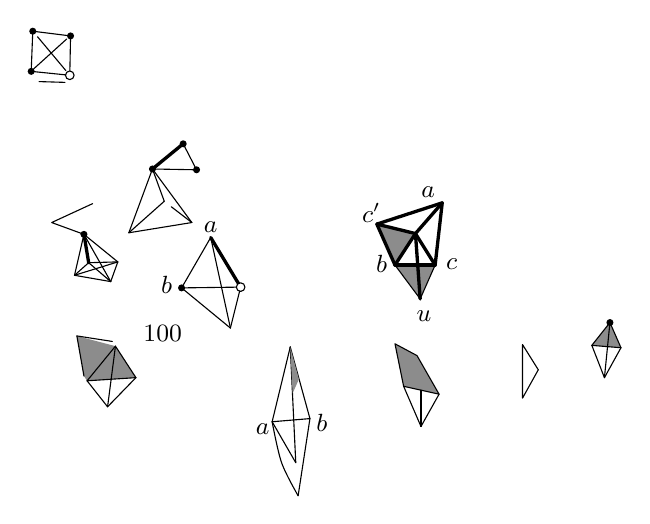
\begin{tikzpicture}[x=1mm,y=1mm,line cap=round,line join=round,font=\scriptsize]
\draw (9.8,-3.8) -- (14.6,-4.4) -- (14.5,-9.4) -- (9.6,-8.9) -- cycle;
\draw (10.4,-4.5) -- (14,-8.8);
\draw (14.1,-4.8) -- (9.9,-8.6);
\draw (10.6,-10.2) -- (13.9,-10.3);
\node[pt] at (9.8,-3.8) {};
\node[pt] at (14.6,-4.4) {};
\node[pt] at (9.6,-8.9) {};
\node[opt] at (14.5,-9.4) {};
\draw[very thick] (25,-21.3) -- (28.9,-18.1);
\draw (28.9,-18.1) -- (30.6,-21.4);
\draw (25,-21.3) -- (30.6,-21.4);
\draw (25,-21.3) -- (22,-29.4);
\draw (25,-21.3) -- (30,-28.1);
\draw (22,-29.4) -- (30,-28.1);
\draw (22,-29.4) -- (26.5,-25.4);
\draw (25,-21.3) -- (26.5,-25.4);
\draw (27.4,-26.1) -- (30,-28.1);
\node[pt] at (28.9,-18.1) {};
\node[pt] at (30.6,-21.4) {};
\node[pt] at (25,-21.3) {};
\draw (17.4,-25.7) -- (12.2,-28.1) -- (16.3,-29.6);
\draw[very thick] (16.3,-29.6) -- (16.9,-33.2);
\draw (16.3,-29.6) -- (15.1,-34.8);
\draw (16.3,-29.6) -- (20.6,-33.1);
\draw (16.3,-29.6) -- (19.7,-35.6);
\draw (15.1,-34.8) -- (19.7,-35.6);
\draw (19.7,-35.6) -- (20.6,-33.1);
\draw (20.6,-33.1) -- (16.9,-33.2);
\draw (16.9,-33.2) -- (15.1,-34.8);
\draw (15.1,-34.8) -- (20.6,-33.1);
\draw (16.9,-33.2) -- (19.7,-35.6);
\node[pt] at (16.3,-29.6) {};
\draw (32.4,-30) -- (28.7,-36.4);
\draw (28.7,-36.4) -- (36.2,-36.3);
\draw (32.4,-30) -- (34.9,-41.5);
\draw (28.7,-36.4) -- (34.9,-41.5);
\draw (36.2,-36.3) -- (34.9,-41.5);
\draw[very thick] (32.4,-30) -- (36.2,-36.3);
\node[pt] at (28.7,-36.4) {};
\node[opt] at (36.2,-36.3) {};
\node[inner sep=1pt] at (32.4,-28.7) {\small $a$};
\node[inner sep=1pt] at (26.8,-36) {\small $b$};
\fill[pattern=north east lines,pencil] (15.4,-42.5) -- (20.3,-43.8) -- (16.7,-48.2) -- (16.3,-47.6) -- cycle;
\fill[pattern=north east lines,pencil] (20.3,-43.8) -- (22.9,-47.8) -- (16.7,-48.2) -- cycle;
\draw (15.4,-42.5) -- (19.9,-43.2);
\draw (15.4,-42.5) -- (16.3,-47.6);
\draw (20.3,-43.8) -- (22.9,-47.8);
\draw (20.3,-43.8) -- (16.7,-48.2);
\draw (20.3,-43.8) -- (19.3,-51.5);
\draw (16.7,-48.2) -- (22.9,-47.8);
\draw (22.9,-47.8) -- (19.3,-51.5);
\draw (16.7,-48.2) -- (19.3,-51.5);
\draw (42.5,-43.9) -- (40.2,-53.4);
\draw (42.5,-43.9) -- (45,-53);
\draw (40.2,-53.4) -- (45,-53);
\draw (42.5,-43.9) -- (43.2,-58.6);
\draw (40.2,-53.4) -- (43.2,-58.6);
\draw (45,-53) -- (43.5,-62.8);
\draw plot[smooth, tension=0.55] coordinates {(40.2,-53.4) (41.4,-58.6) (43.5,-62.8)};
\fill[pattern=north east lines,pencil] (42.5,-43.9) -- (43.6,-48) -- (42.8,-49.8) -- cycle;
\node[inner sep=1pt] at (39,-54.3) {\small $a$};
\node[inner sep=1pt] at (46.5,-53.6) {\small $b$};
\fill[pattern=north east lines,pencil] (53.5,-28.3) -- (58.4,-29.5) -- (55.8,-33.5) -- cycle;
\fill[pattern=north east lines,pencil] (55.8,-33.5) -- (60.9,-33.5) -- (59,-37.8) -- cycle;
\draw[very thick] (53.5,-28.3) -- (61.8,-25.6);
\draw[very thick] (53.5,-28.3) -- (58.4,-29.5);
\draw[very thick] (61.8,-25.6) -- (58.4,-29.5);
\draw[very thick] (58.4,-29.5) -- (55.8,-33.5);
\draw[very thick] (58.4,-29.5) -- (60.9,-33.5);
\draw[very thick] (58.4,-29.5) -- (59,-37.8);
\draw[very thick] (55.8,-33.5) -- (60.9,-33.5);
\draw[very thick] (53.5,-28.3) -- (55.8,-33.5);
\draw[very thick] (61.8,-25.6) -- (60.9,-33.5);
\draw (55.8,-33.5) -- (59,-37.8);
\draw (60.9,-33.5) -- (59,-37.8);
\node[inner sep=1pt] at (52.8,-26.9) {\small $c'$};
\node[inner sep=1pt] at (60,-24.2) {\small $a$};
\node[inner sep=1pt] at (54.1,-33.4) {\small $b$};
\node[inner sep=1pt] at (63,-33.4) {\small $c$};
\node[inner sep=1pt] at (59.5,-40) {\small $u$};
\fill[pattern=north east lines,pencil] (55.8,-43.5) -- (58.6,-45) -- (61.4,-49.9) -- (56.9,-48.9) -- cycle;
\draw (55.8,-43.5) -- (58.6,-45) -- (61.4,-49.9) -- (56.9,-48.9) -- cycle;
\draw (56.9,-48.9) -- (59.1,-54);
\draw (61.4,-49.9) -- (59.1,-54);
\draw (59.1,-49.4) -- (59.1,-54);
\draw (72,-43.6) -- (74,-46.8) -- (72,-50.4) -- cycle;
\fill[pattern=north east lines,pencil] (83.1,-40.8) -- (80.8,-43.7) -- (84.5,-44) -- cycle;
\draw (83.1,-40.8) -- (80.8,-43.7);
\draw (83.1,-40.8) -- (84.5,-44);
\draw (80.8,-43.7) -- (84.5,-44);
\draw (80.8,-43.7) -- (82.4,-47.8);
\draw (84.5,-44) -- (82.4,-47.8);
\draw (83.1,-40.8) -- (82.4,-47.8);
\node[pt] at (83.1,-40.8) {};
\node[inner sep=1pt] at (26.3,-42.2) {\small 100};
\end{tikzpicture}
\end{document}
